\begin{center}
\fbox{\fbox{\parbox{6.5in}{\centering
\begin{flushleft}

\vspace{2mm}
\hspace{5mm}
NB! Enne peatükki uurimist on soovituslik endale selgeks teha peatükk \ref{peatükk_8}.

\vspace{5mm}
\hspace{5mm}
\textbf{\underline{Kahe tundmatuga lineaarvõrrandisüsteem}}

\vspace{2mm}
\hspace{5mm}
Võib esineda ülesandeid, mis nõuavad et oleks rahuldatud mitu erinevat lineaarvõrrandit (teisisõnu ka\\ \hspace{5mm} mitu erinevat tingimust).
Mõlemad võrrandid peavad kehtima samade $x$ ja $y$ väärtuste korral ja\\ \hspace{5mm} moodustavad selleõttu lineaarvõrrandisüsteemi, mida üldiselt tähistatakse nõnda:

\begin{equation}
\label{25_eq1}
\begin{cases}
y=a_{1}x+b_{1}\\
y=a_{2}x+b_{2}
\end{cases}
\end{equation}

\vspace{2mm}
\hspace{5mm}
kus $a_{1}$, $b_{1}$, $a_{2}$ ja $b_{2}$ on suvalised arvkordajad (arvud), ning $x$ ja $y$ on tundmatud.

\vspace{2mm}
\hspace{5mm}
Lahendiks peavad tulema sellised $x$ ja $y$ väärtused, mis sobivad nii esimesse kui teisse võrrandisse (ehk\\ \hspace{5mm} mõlema võrrandi puhul peab $VP=PP$).

\vspace{2mm}
\hspace{5mm}
\textbf{Näiteks:}

\vspace{2mm}
\hspace{5mm}
Olgu meil järgmine kahe tundmatuga lineaarvõrrandisüsteem:

\[ \begin{cases}
y=3x+2\\
y=-7x+1
\end{cases} \]

\hspace{5mm}
Kui valida sellised $x$ ja $y$ väärtused, mis rahuldavad vaid esimest võrrandit, siis leiame, et need samad\\ \hspace{5mm} lahendid ei pruugi teise võrrandi jaoks sobivad olla. Võtame näiteks esimese võrrandi lahenditeks $x=1$\\ \hspace{5mm} ja seega $y=3\cdot 1 +2=5$. 

\vspace{2mm}
\hspace{5mm}
Esimese võrrandi puhul võrdub vasak pool parema poolega küll, kuid kas samad $x$ ja $y$ väärtused\\ \hspace{5mm} sobivad teise võrrandi lahendiks?

\vspace{2mm}
\hspace{5mm}
Asetame $x=1$ ja $y=5$ teisse võrrandisse ja kontrollime.

\begin{equation}
\label{25_eq2}
y = -7x+1 \longrightarrow \left[ \begin{tabular}{c}
$x=1$\\
$y=5$
\end{tabular} \right] \longrightarrow 5=-7 \cdot 1 +1 \longrightarrow 5=-6
\end{equation}

\hspace{5mm}
Saime, et $5\neq -6$ ehk $VP \neq PP$, mis tähendab et need $x$ ja $y$ väärtused selle süsteemi jaoks ei sobinud.\\ \hspace{5mm} Sobivate väärtuste leidmist vaatleme järgmistes peatükkides, kuid muidu lahendid sellise süsteemi\\ \hspace{5mm} jaoks on $x=\dfrac{1}{4}$ ja $y=\dfrac{11}{4}$.

\vspace{5mm}
\hspace{5mm}
\textbf{\underline{Lineaarvõrrandisüsteemi graafiline lahendamine}}

\vspace{2mm}
\hspace{5mm}
Esimene meetod, kuidas võrrandisüsteemi jaoks lahendit leida, on need võrrandid välja joonistada ning\\ \hspace{5mm} leida punkt, kus sirged lõikuvad (teisisõnu leiame ühise punkti, mis kuulub mõlemale võrrandile).

\vspace{2mm}
\hspace{5mm}
Meenutame, et punkti asukoht graafikul oli määratud $x$-iga ja $y$-iga: 

\begin{itemize}
\item $x$ - kui palju tuleb liikuda nullist vasakule või paremale
\item  $y$ - kui palju tuleb liikuda nullist ülesse või alla
\end{itemize}


\end{flushleft}
}}}
\end{center}

\pagebreak

\begin{center}
\fbox{\fbox{\parbox{6.5in}{\centering
\begin{flushleft}

\vspace{2mm}
\hspace{5mm}
\textbf{Näiteks:}

\vspace{2mm}
\hspace{5mm}
Vaatleme järgmist lineaarvõrrandisüsteemi:

\begin{equation}
\label{25_eq3}
\begin{cases}
2x+5y=10\\
-3x+15y=1
\end{cases}
\end{equation}

\hspace{5mm}
Esmalt tuleb meil võrrandid viia sellisele kujule nagu avaldises \ref{25_eq1}. Ehk avaldame $y$ väärtused $x$-i\\ \hspace{5mm} kaudu.

\vspace{2mm}
\hspace{5mm}
Alustame võrrandist $2x+5y=10$.

\hspace{5mm}
Jätame vasakule poole võrdust vaid $y$-id ja muud asjad viskame teisele poole võrdusmärki. Saame:
\[ 5y=10-2x \]

\vspace{2mm}
\hspace{5mm}
Nüüd et $y$ ees olevast kordajast ($5$-st) lahti saada, jagame mõlemad võrduse pooled 5-ga läbi (või\\ \hspace{5mm} korrutame $\dfrac{1}{5}$-ga läbi). Saame:

\[5y \cdot \dfrac{1}{5} = 10 \cdot \dfrac{1}{5}-2x \cdot \dfrac{1}{5}  \hspace{3mm} \longrightarrow \hspace{3mm} y=2-\dfrac{2x}{5} \]


\vspace{5mm}
\hspace{5mm}
Nüüd võrrand $-3x+15y=1$. 

\hspace{5mm}
Samamoodi, jätame $y$-id vasakule ja muud asjad paremale. Saame:

\[ 15y=1+3x \]

\hspace{5mm}
Et $15$-st lahti saada $y$ ees, siis jagame kogu avaldise $15$-ga läbi. Saame:

\[ 15y\cdot \dfrac{1}{15}=1\cdot \dfrac{1}{15}+3x\cdot \dfrac{1}{15} \hspace{3mm} \longrightarrow \hspace{3mm} y=\dfrac{1}{15}+\dfrac{x}{5} \] 

\hspace{5mm}
Nüüd näeb meie võrrandisüsteem välja nõnda:

\begin{equation}
\label{25_eq4}
\begin{cases}
y= 2- \dfrac{2x}{5}\\
y=\dfrac{1}{15}+\dfrac{x}{5}
\end{cases}
\end{equation}

\hspace{5mm}
Nüüd joonestame ühele ja samale teljestikule mõlemad võrrandi graafikud \ref{peatükk_8}.nda peatükki eeskirja järgi. 

\begin{center}
\includegraphics[scale=0.5]{"25_linsys_graph_joonis.png"}
\label{25_joonis1}
\captionof{figure}{Võrrandite lõikumispunkt}
\end{center}

\end{flushleft}
}}}
\end{center}

\begin{center}
\fbox{\fbox{\parbox{6.5in}{\centering
\begin{flushleft}

\vspace{2mm}
\hspace{5mm}
Nagu jooniselt \ref{25_joonis1} näha, lõikuvad meil sirged ligikaudu punktis $(3.2, 0.7)$. See tähendab, et meie\\ \hspace{5mm} lineaarvõrrandisüsteemi lahend ongi ligikaudu $x=3.2$ ja $y=0.7$. Ehk:

\[ \begin{cases}
x=3.2\\
y=0.7
\end{cases} \]

\vspace{2mm}
\hspace{5mm}
Kuid ligikaudsed lahendid ei ole piisavalt täpsed, mille tõttu jääb praegune meetod järgmistele\\ \hspace{5mm} meetoditele alla. Graafiliselt on tore lahendeid leida, kui punktid asuksid mingite kindlate graafikul\\ \hspace{5mm} märgitud jaotiste peal. Kohe kui punkt on graafiku telgedele märgitud jaotise väärtustelt veidi maas,\\ \hspace{5mm} siis tekkib silmaga väärtuse määramisel viga sisse.

\vspace{5mm}
\hspace{5mm}
Tasuks ka mainida kahte juhtu graafilise lahendamise puhul:

\vspace{2mm}
\hspace{5mm}
1) \textbf{Kui lineaarvõrrandisüsteemi võrranditele vastavad graafikud on \underline{paralleelsed} sirged, siis\\ \hspace{5mm} võrrandisüsteemil lahend puudub. Võrrandisüsteemi nimetatakse vasturääkivaks.\\ \hspace{5mm} (vt joonist \ref{25_joonis2}).}

\vspace{2mm}
\hspace{5mm}
2) \textbf{Kui lineaarvõrrandisüsteemi võrranditele vastavad graafikud on \underline{kattuvad sirged} (nad\\ \hspace{5mm} on üksteise peal), siis on süsteemil lõpmatult palju lahendeid. (vt joonist \ref{25_joonis3}).}


\begin{minipage}{7cm}
	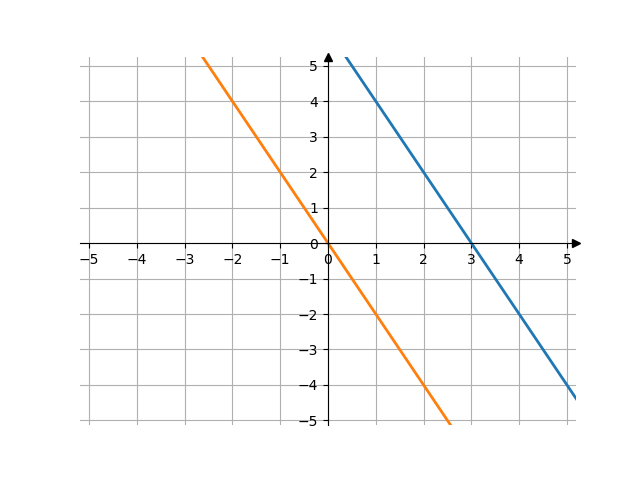
\includegraphics[width=7cm]{25_joonis2.png}
	\captionof{figure}{Paralleelsed sirged}
	\label{25_joonis2}
\end{minipage}
\hspace{.05\linewidth}
\begin{minipage}{.45\linewidth}
	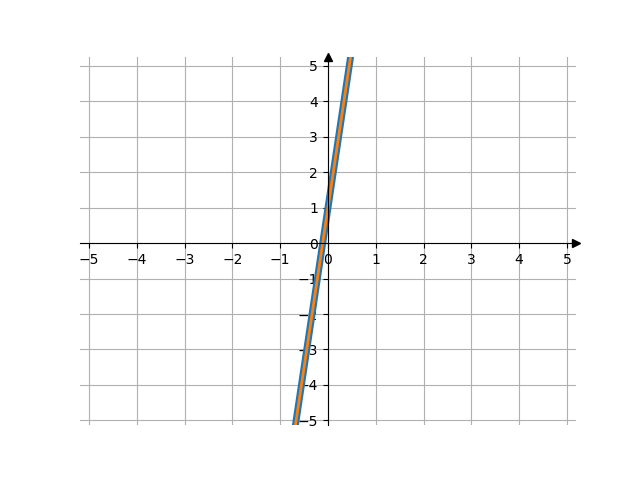
\includegraphics[width=7cm]{25_joonis3.png}
	\captionof{figure}{Kattuvad sirged}
	\label{25_joonis3}
\end{minipage}

\end{flushleft}
}}}
\end{center}


\vspace{0.5cm}

\textbf{Märkmed}\\
\vspace{2mm}
\begin{mdframed}[style=graphpaper]
\vspace{6cm}
\end{mdframed}


\pagebreak
\vspace{0.5cm}

\textbf{Märkmed}\\
\vspace{2mm}
\begin{mdframed}[style=graphpaper]
\vspace{21cm}
\end{mdframed}